% !TeX spellcheck = en_US
\documentclass[10pt,a4paper, notitlepage]{report}
\usepackage[english]{babel}
\usepackage[latin1]{inputenc}
\usepackage{amsmath}
\usepackage{amsfonts}
\usepackage{amssymb}
\usepackage{epstopdf}
\usepackage{graphicx}
\usepackage{caption}
\usepackage{subcaption}
\usepackage{hyperref}
\usepackage{float}
\usepackage{lettrine}
\usepackage{lipsum}
\usepackage{xcolor}
\usepackage{listings}

\definecolor{mGreen}{rgb}{0,0.6,0}
\definecolor{mGray}{rgb}{0.5,0.5,0.5}
\definecolor{mPurple}{rgb}{0.58,0,0.82}
\definecolor{backgroundColour}{rgb}{0.95,0.95,0.92}


\lstdefinestyle{CStyle}{
  backgroundcolor=\color{backgroundColour},   
  commentstyle=\color{mGreen},
  keywordstyle=\color{magenta},
  numberstyle=\tiny\color{mGray},
  stringstyle=\color{mPurple},
  basicstyle=\footnotesize,
  breakatwhitespace=false,         
  breaklines=true,                 
  captionpos=b,                    
  keepspaces=true,                 
  numbers=left,                    
  numbersep=5pt,                  
  showspaces=false,                
  showstringspaces=false,
  showtabs=false,                  
  tabsize=2,
  language=C
}

\newcommand{\superref}[3]{\hyperref[#1]{#2} (\capitalisewords{#3} \ref{#1})}

\title{Modular Software for a Wheeled Robot:\\SRRG Orazio Core on dsPIC}
\author{Irvin Aloise, Mirco Colosi\\ \tt\small \{ialoise, colosi\}@diag.uniroma1.it}

\begin{document}
\maketitle


\textbf{Keywords.} \textit{Mobile Robotics, Microcontrollers, Software Development}

\section*{Introduction} \label{sec:intro}
\lettrine{S}{}mall robots used in educational robotics typically adopt a microcontroller to execute time critical tasks and interact with the physical hardware. In fact, small boards that embed a microcontroller are tailored for this job, since they allow to directly interface the microcontroller with a wide range of peripherals. Moreover - in general - the cost of those components is relatively low, so this helps to keep the system cheap and allows to a broad range people - e.g. students - to build their own mobile robot.

The Orazio robot is a wheeled robot developed within the Ro.Co.Co. Laboratory of Sapienza University that matches this philosophy. It is designed to be built by students (bachelor and high-school ones) and for this reason it is modular, simple and cheap, even if it can be used for more complex tasks or for testing robotics algorithms and systems. The Orazio software has been also developed with those concepts in mind and so it is fully modular and compact. The software offers high level interfaces so that upper layers are independent from the implementation of the lower ones. This modularity allow us to isolate the layer that interacts with the microcontroller, leading to the possibility of changing architecture without touching the remaining parts.

\begin{figure}[!h]
  \centering
  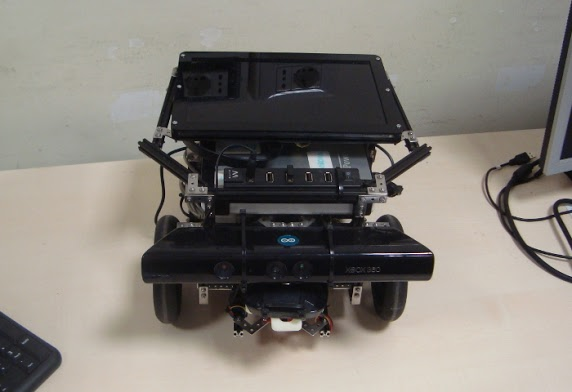
\includegraphics[width=0.75\linewidth]{pics/orazio}
  \caption{The Orazio robot built by a master student. In this unit, there is also a Microsoft Kinetic that will stream RGB-D images on an external PC.}
  \label{fig:orazio}
\end{figure}

On the basis of this, in our project we extended the Orazio software to include also the \texttt{dsPIC33f} microcontroller. We opted for this architecture because it performs in hardware the processing of encoder data: since this can be sampled at very high rates - even 400~kHz - this feature will reduce the load on the actual MCU.

The remaining of this document is organized as follows: firstly, we provide a brief overview of the low level layer - i.e. the one that actually manages the MCU and its peripherals; then we will go with an introduction on the other layers and a sketch of the client that runs on an external device; finally the conclusions and future works of related to this project.

\section*{Orazio Software Implementation} \label{sec:approach}
In this section we provide an overview of the Orazio software, starting from the \textit{bare-metal} level to the client that runs on the user's PC. Obviously the software is completely open-source and can be downloaded from our repository~\footnote{\href{https://gitlab.com/srrg-software/srrg2_orazio_core.git}{https://gitlab.com/srrg-software/srrg2\_orazio\_core.git}}. The repository contains the full software that runs on Orazio together with the unit tests for each of the peripherals developed.
\subsection*{Low Level Layer}
The board we used in this project is the \textit{MuIn dsNav}, an open-source platform developed for small robotics applications. Figure~\ref{fig:dsnav} illustrates the board and its output pins.

The MCU embedded on this board is the \texttt{dsPIC33FJ128MC802}~\footnote{\href{https://www.microchip.com/wwwproducts/en/dspic33fj128mc802}{https://www.microchip.com/wwwproducts/en/dspic33fj128mc802}}. It has a 16-bit architecture, a max clock speed of 40 MHz and 16 KB of SRAM. This version designed with the \texttt{MC} acronym - i.e. Motor Controller - has 8 PWM output and 2 Quadrature Encoder Interface that make this MCU tailored for a differential drive robot, since they have only 2 actuators.

\begin{figure}[!h]
  \centering
  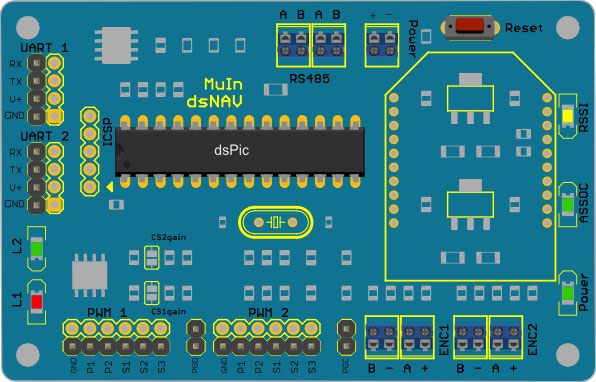
\includegraphics[width=0.6\linewidth]{pics/dsnav_simple}
  \caption{The board used in the project: MuIn dsNav. Notice the pin outputs for encoders and PWMs.}
  \label{fig:dsnav}
\end{figure}

In order to make the robot fully functional we had to develop a set of peripherals, so in this sub-section we will provide some hints about how each of them works.
% -------------------------------------------------------------------------------
\paragraph*{UART}
When developing software for a microcontroller, the first thing to implement is the communication. In this way it is possible to send and receive data from the PC, allowing to debug the system if something is not behaving properly. 
The defaul UART baud rate here is set to 115200 Bd, however it can be adjusted to other values. The transmission is handled through interrupts in order to avoid the waste of resources. The functionalities offered to the higher layers are simple and easy to understand:
\begin{itemize}
  \item[--] \texttt{UART\_init}: this function sets up the UART control registers, pin configuration and enables the communication.
  \item[--] \texttt{UART\_putChar}: transmits a character from the MCU to the receiver; the operation is performed atomically - i.e. disabling all the interrupts while operating.
  \item[--] \texttt{UART\_getChar}: receives a character from the external PC; the routine is blocking but the operation is performed atomically.
\end{itemize}
% -------------------------------------------------------------------------------
\paragraph*{Timers}
A timer is useful to handle time-related operations - e.g. a watchdog for the platform. The \texttt{dsPIC33F} has three types of timers on the basis of their functionalities: named Type A (Timer 1), Type B (Timer 2-4-6-8) and Type C (Timer 3-5-7-9). Each one is 16-bit timer, however Type B and Type C can be grouped to emulate a 32-bit counter. In our configuration we hook to Timer 3 with a duration that can be configured by the user. In this configuration, a \texttt{Timer} has a pointer to the function that will handle the interrupt, adding more freedom to the peripheral behavior. Again, the functionalities offered to the upper layer are simple and minimalistic:
\begin{itemize}
  \item[--] \texttt{Timer\_create}: creates a timer with a specified period; in this phase the user must also indicate the function that will be called in the ISR.
  \item[--] \texttt{Timer\_start} and \texttt{Timer\_stop}: enable or disable the related interrupt.
  \item[--] \texttt{Timer\_destroy}: stops and destroys the configuration of a previously created timer.
\end{itemize}
% -------------------------------------------------------------------------------
\paragraph{Digital I/O} In the Orazio firmware we consider generic pins that have a digital outputs as peripherals. In this sense, a digital pin will have a \textit{direction} - i.e. input or output - and a \textit{value}. The structure \texttt{Pin} is at the basis of this peripherals so a suited configuration of this must be done in advance. In particular, we have to set the input, output and direction register together with the pin number. In the selected MCU, for digital IO pins, those are pointers to the following registers:
\begin{itemize}
  \item \texttt{input\_reg} $\rightarrow$ \texttt{PORTB}
  \item \texttt{output\_reg} $\rightarrow$ \texttt{LATB}
  \item \texttt{direction\_reg} $\rightarrow$ \texttt{TRISB}
\end{itemize}
Summarizing, a certain \texttt{Pin} will be mapped into a related bit in those registers. The functionalities offered are:
\begin{itemize}
  \item[--] \texttt{DigIO\_init}: initialize each digital pin, clearing the value (pull-up) and the direction (input).
  \item[--] \texttt{DigIO\_setDirection} and \texttt{DigIO\_getDirection}: simple setter and getter of the pin direction.
  \item[--] \texttt{DigIO\_setValue} and \texttt{DigIO\_setValue}: setter and getter of the pin value.
\end{itemize}
% -------------------------------------------------------------------------------
\paragraph{EEPROM} The \texttt{dsPIC33F} has a flash non-volatile memory. However, to keep things consistent with the other architectures supported, we developed an EEPROM peripheral. The emulation is obtained through a small library provided by Microchip itself~\footnote{\href{https://bit.ly/2GnH1KN}{https://bit.ly/2GnH1KN}} that maps EEPROM to Program Memory. This makes the EEPROM implementation relatively easy:
\begin{itemize}
  \item[--] \texttt{EEPROM\_init}: initializes the emulator subsystem.
  \item[--] \texttt{EEPROM\_read}: reads a specified number of bytes starting from a specific index in the memory.
  \item[--] \texttt{EEPROM\_write}: writes a specified number of bytes starting from a specific index in the memory.
\end{itemize}
% -------------------------------------------------------------------------------
\paragraph{Encoders} As we already stated before, the MCU we selected has 2 Quadrature Encoder Interfaces (QEIs) that allow hardware processing of the data coming from those sensors. In this sense, sampling data from an encoder will translate in a simple read of a specific QEI register. The resulting APIs are the following:
\begin{itemize}
  \item[--] \texttt{Encoder\_init}: initializes the QEIs control registers and maps the relative pins.
  \item[--] \texttt{Encoder\_sample}: samples the value of both encoders, atomically reading from the QEI register the values.
  \item[--] \texttt{Encoder\_getValue}: returns the last sampled value.
\end{itemize}
% -------------------------------------------------------------------------------
\paragraph{Pulse Width Modulation} The generation of analog commands from digital values is called Pulse Width Modulation - shortened as PWM. In this case, we use it to control the amount of power supplied to the motors. The MCU can generate a pulse wave with a specific period; what we control is the \textit{duty cycle}, which describes the proportion of 'up' time of the wave. A higher duty cycle translates into more power supplied to motors. 
However, to drive a robot we also need to specify the direction of the motion. In this case the H-Bridge that we implemented requires an analog input that represents the amount of power to supply to the motor, together with a digital value (0 or 1) that indicates the direction of the motion. 
Although Orazio supports different H-Bridge implementations, for the dsPIC we only support the PWM + Direction one. Moreover to keep the whole Orazio software consistent, we reduced the granularity of PWM values to 255 - instead of 4096.
The resulting API for this sub-module is the following:
\begin{itemize}
  \item[--] \texttt{PWM\_init}: initializes the subsystem, setting up the PWM control registers and the number of channels that we use.
  \item[--] \texttt{PWM\_enable}: enables the PWM on the specified channel.
  \item[--] \texttt{PWM\_setDutyCycle} and \texttt{PWM\_getDutyCycle}: sets/gets the duty cycle for a specific PWM channel.
\end{itemize}
What it is good to notice is that the pins used as PWM are analog, therefore the pointers to \texttt{input\_reg}, \texttt{output\_reg} and \texttt{direction\_reg} are \texttt{NULL}. Instead, we have to specify the Output Compare and the Counter registers, which are the following:
\begin{itemize}
  \item \texttt{oc\_reg} $\rightarrow$ \texttt{P1DCx} where \texttt{x} stands for the channel (can be 1 or 2).
  \item \texttt{tcc\_reg} $\rightarrow$ \texttt{PWM1CON1}
\end{itemize}
In the Appendix of this document we provide the full pin configuration for this architecture.

\vspace{10px}
Given this brief overview of the low-level APIs and their implementation for the Microchip MCU, we can now go through the higher level parts of the Orazio software.

% -------------------------------------------------------------------------------
\subsection*{Orazio Architecture}
Once that the system can manage properly all its peripherals, we can now start to analyze how the whole Orazio system works.

\begin{figure}[!h]
  \centering
  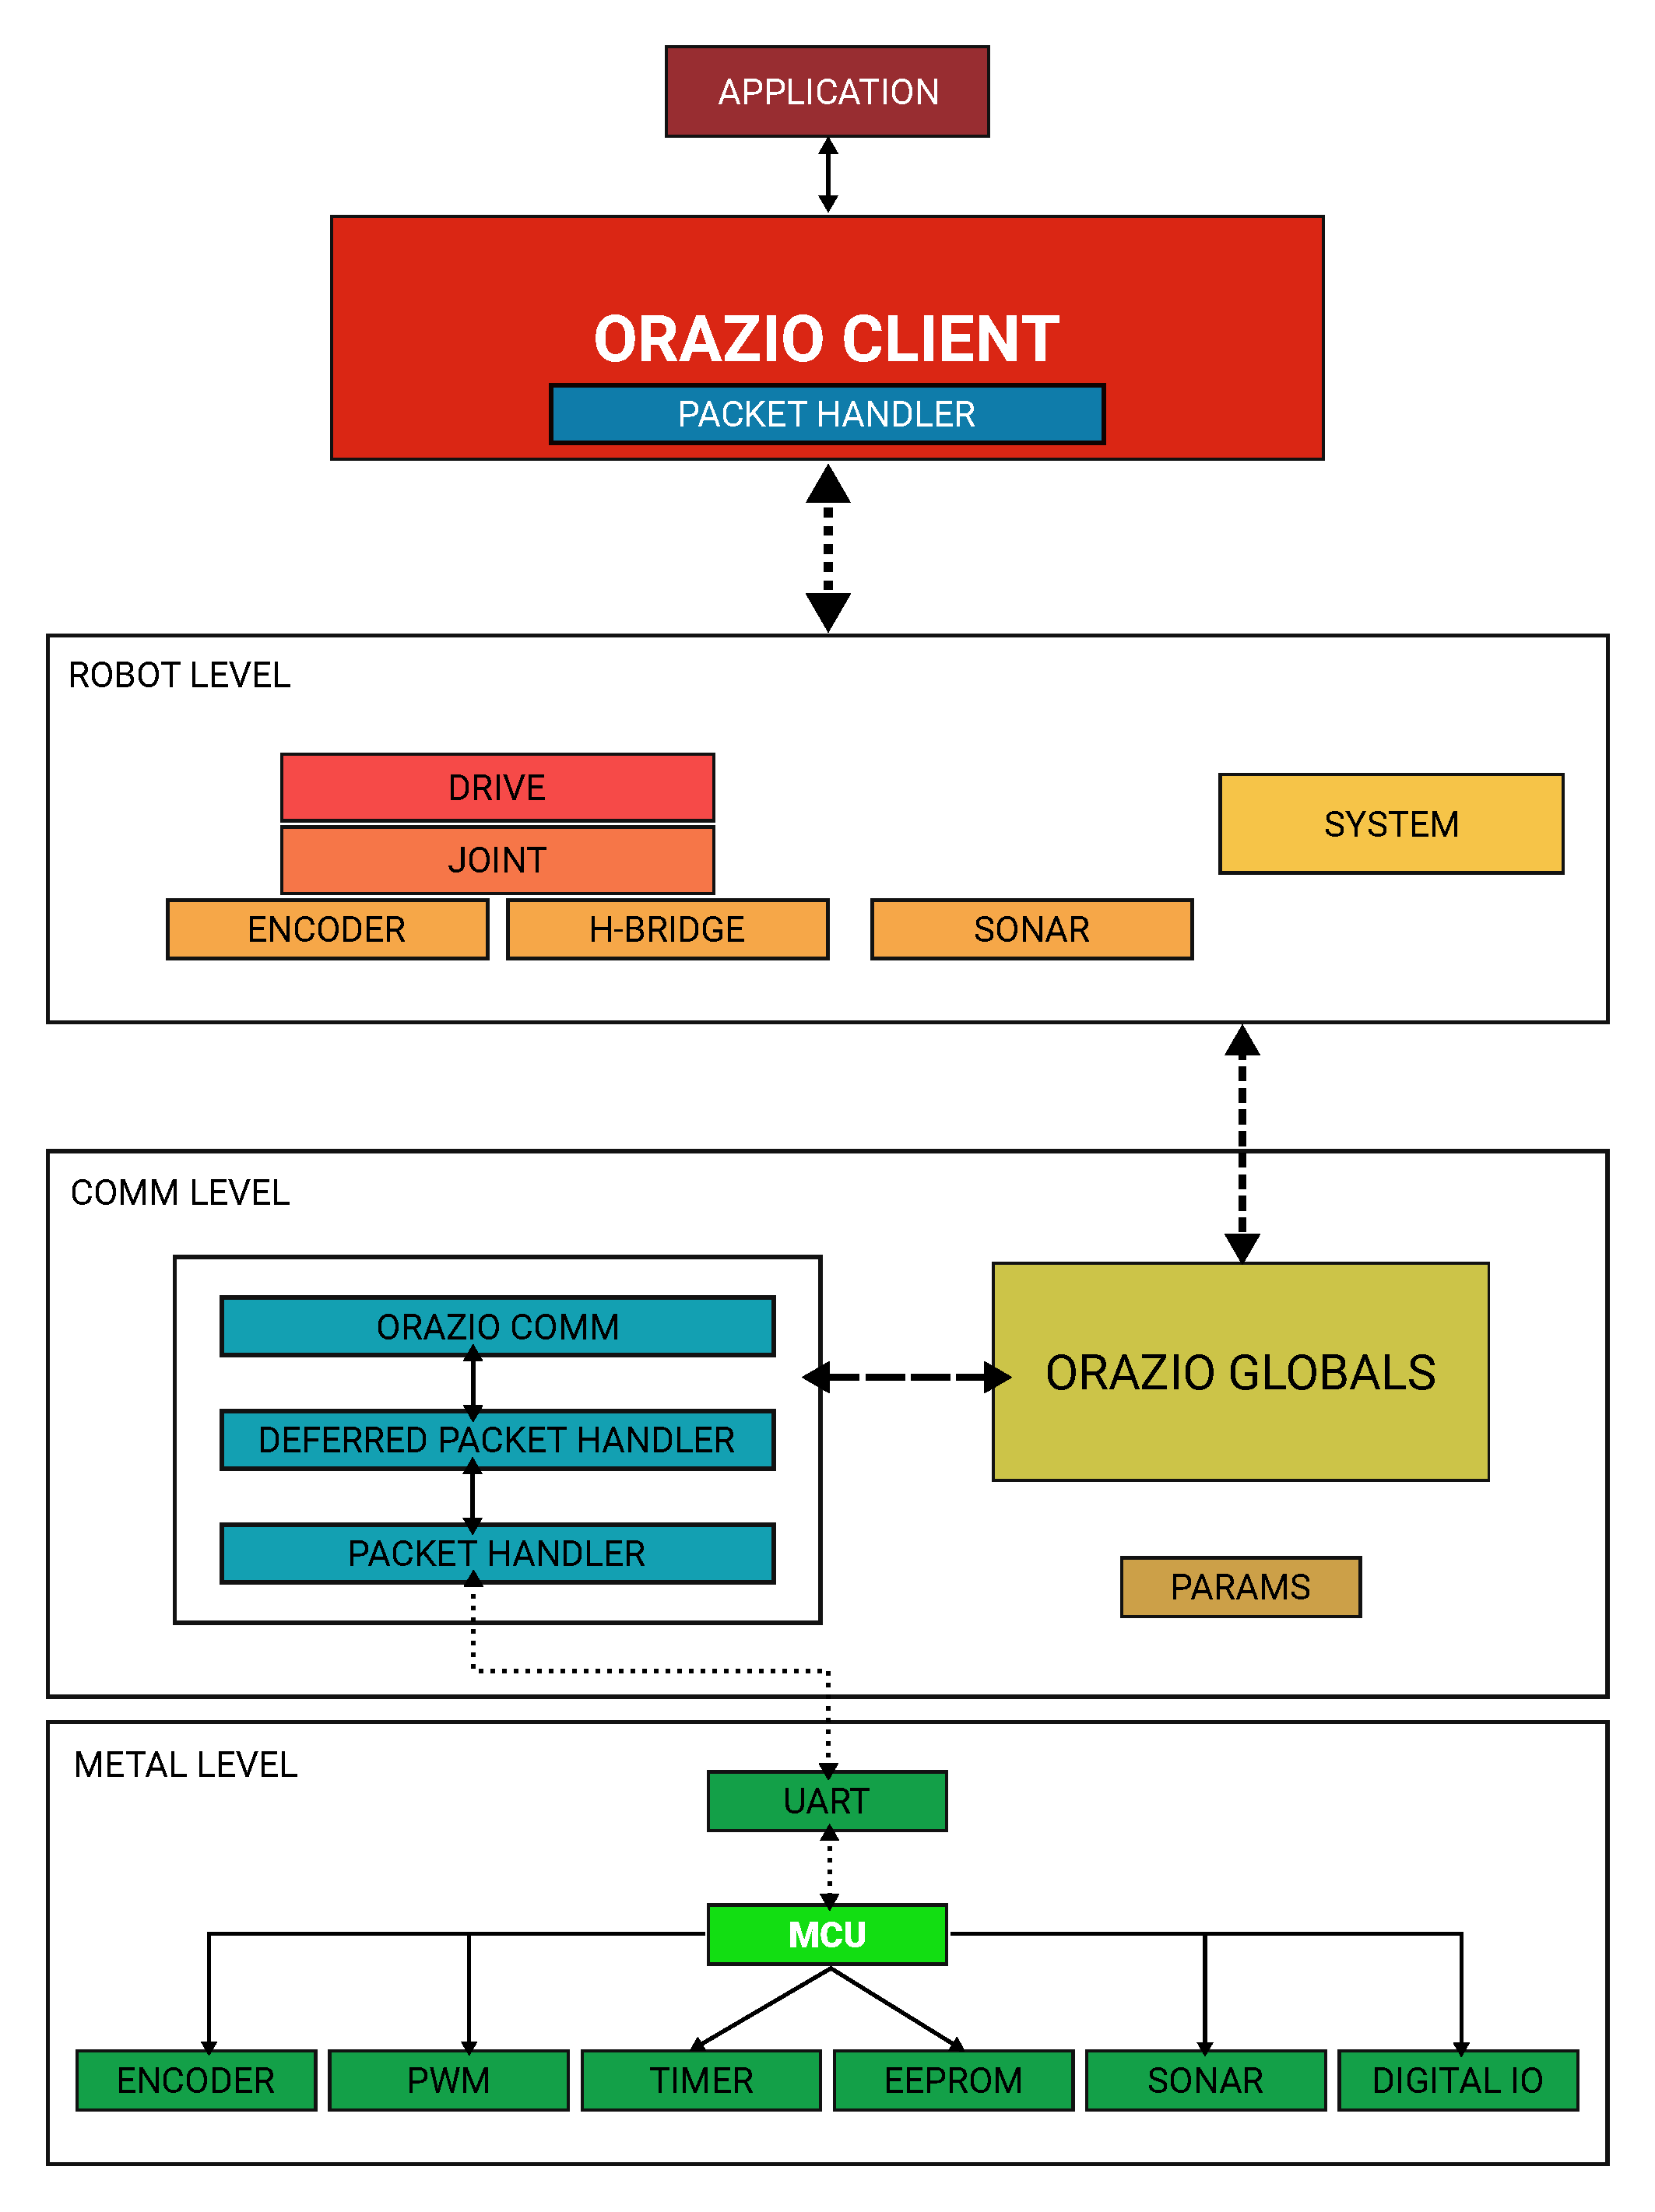
\includegraphics[width=0.8\linewidth]{pics/orazio_arch}
  \caption{Orazio software architecture. The client can be attached to different applications. What we provide by default is a web-socket that together with a shell sends the platform logging to the browser.}
  \label{fig:orazio_arch}
\end{figure}

The MCU gather all data generated on the board (both internally and from sensors) and sends them to the user PC. Therefore the MCU acts like a server that broadcasts the information to the client connected. The client on its side can send data to the MCU - e.g. set some parameters. Figure~\ref{fig:orazio_arch} illustrates the whole architecture and te connections between the sub-modules.

\paragraph{Orazio Communications} The communication is carried on through a packet protocol: each different 'topic' will have its own packet - e.g. \texttt{SystemPacket}, \texttt{JointStatusPacket} and so on. The MCU imposes the timing of the communication periodically sending an \texttt{EndEpochPacket}.

In order to inform the client that a new packet is coming, the MCU sends the token \texttt{0xAA55}. In this way, the client hooks the packet and can decode it. The entity in charge of managing the packets is the \texttt{PacketHandler}. Orazio will also have a \texttt{DeferredPacketHandler} built on top of the previous: in this way it is possible to accumulate packets in a queue and periodically process them. In order to handle a new type of packet, we have to install the designated packet in the \texttt{PacketHandler}, specifying the operation that will performed when such packet will be received - i.e. a function pointer. Summarizing, the communication epoch starts with the \texttt{0xAA55} token, goes on with the retrieval of the packet information (type, size, ...), gets the actual payload and finally reads the checksum; the end of an epoch is imposed by the \texttt{EndEpochPacket}. All of this is performed with a finite state machine implemented through function pointers. More information on this topic can be found in the files \texttt{packet\_handler.h} and \texttt{packet\_handler.c}.

\paragraph{Orazio Globals} The interaction between MCU and client will involve a set of global variables - located in \texttt{orazio\_globals.h}. Those global variables store the configuration, state and control of each subsystem. Therefore each time the client asks for or tries to set something, those variables will be involved - since all modules interact though those global variables.

\paragraph{Orazio Sub-Systems} An aggregation of variables represents a subsystem of the robot - e.g. \texttt{Sonar}, \texttt{DifferentialDrive} and so on. Those are high-level structures that allow also to do be composed - e.g. \texttt{Joint} is a combination of \texttt{Encoder} and \texttt{H\_Bridge} - and to perform some processing - e.g. motor PIDs and odometry retrieval from encoder ticks.

\paragraph{Orazio Configuration} In order to set a robot parameter - e.g. PID gains - the client has to \textit{send} it to the MCU and the value will be stored in MCU memory. However, some of the parameters will remain unchanged for the entire robot life - e.g. the baseline - and, therefore, it would be useful to avoid set them each time. For this reason, once that the client sends a parameter, it can also ask to \textit{store} it: in this case the MCU will save the parameter in the non-volatile memory - i.e. EEPROM or Flash.
The same is also valid for the reading process: the client can perform a \textit{fetch} from the MCU memory or a \textit{request} reading from the non-volatile one. 
In both cases the MCU will send back a \texttt{ResponsePacket} with operation status - i.e. success, failure.

\paragraph{Application} On top of the client, it is possible to develop several applications, depending on the specification that we want to satisfy. In the repository is provided a web-socket that streams the status of the entire system to the browser, allowing also to change and store the configuration on the fly. 

\section*{Conclusions and Future Works} \label{sec:conclusions}
In this project we developed a porting of the Orazio software on the Microchip \texttt{dsPIC33FJ128MC802} MCU.
The modularity of the software allows to change MCU architecture without touching the upper levels, in order to give flexibility to the platform without too much effort. Moreover, since the entire system has been developed with efficiency in mind, performances reach a reasonably high level, leaving room for the addition other modules to the robot.

We targeted the dsPIC architecture in order to exploits some of its features like the hardware decode of encoder streams that make this MCU perfect for a differential drive robot. \textit{The porting is fully functional} and allows to build an Orazio unit with this MCU.

However, what  we notice developing this porting, is that the MCU we choosen is not so powerful in handling a complex software like the Orazio one. For example, other architectures - e.g. ATmega 2560 - are able to run the same software on the same robot with almost twice the number of free cycles - i.e. 2000 free-cycles on the dsPIC vs more than 4000 on the ATmega. For this reason we aim to target more powerful MCU architectures - e.g. ARM ones. 

Moreover, we plan to develop tools to upgrade the robustness of the platform. To this end, a possible future work could be the implementation of a \textit{self-check} module, ensuring in boot phase that each peripheral works properly. In this way it could be possible to avoid runtime failures due to hardware problems, which are frequent when working at a non-industrial level.

\newpage
\section*{Appendix A} \label{sec:appendix}
In this Appendix we show the \texttt{Pin} structure, and the value assigned to each pin in order to properly manage QEI, PWMs and UART. 

A \texttt{Pin} is a structure with the following attributes:
\begin{lstlisting}[style=CStyle]
typedef struct{
  volatile uint16_t* in_register;
  volatile uint16_t* out_register;
  volatile uint16_t* dir_register;
  uint8_t bit;
  
  // timer registers for PWM
  volatile uint16_t* tcc_register;
  volatile uint16_t* oc_register;
  const uint16_t com_mask;
}  Pin;

#define PINS_NUM 14  //for consistency

extern const Pin pins[];
\end{lstlisting}

The value assigned to the pins instead are reported here:
\begin{lstlisting}[style=CStyle]
//ia @brief there are 14RB pins that can be mapped for doing things
//ia they are used for PWMs, encoders and general digital-I/O stuff
//ia RB7 and RB8 are missing since they are used for the UART.

//ia @brief in this implementation we have 
//ia the following pin configuration:
//ia        Encoders: RP10 -> QEA1; RP11 -> QEB1; 
//ia                  RP06 -> QEA2; RP05 -> QEB2; 
//ia        PWM: RP14 -> PWM1H1; RP15 -> PWM1DIR; 
//ia             RP12 -> PWM1H2; RP13 -> PWM2DIR; 
//ia
//ia to select TRISBbits.TRISB15 we will use:
//ia c = 2
//ia const Pin* pin = pins+c;
//ia *pin->dir_register |= (1<<pin->bit)

#include <p33FJ128MC802.h>
#include "pins.h"

const Pin pins[] =
{
  //0
  {
    .in_register=&PORTB,
    .out_register=&LATB,
    .dir_register=&TRISB,
    .bit=0,
    .tcc_register=0,
    .oc_register=0,
    .com_mask=0
  },
  //1
  {
    .in_register=&PORTB,
    .out_register=&LATB,
    .dir_register=&TRISB,
    .bit=1,
    .tcc_register=0,
    .oc_register=0,
    .com_mask=0
  },
  //2 PWM1L1 -> this is used for the direction of the PWM1
  {
    .in_register=&PORTB,
    .out_register=&LATB,
    .dir_register=&TRISB,
    .bit=15,
    .tcc_register=0,
    .oc_register=0,     
    //      .com_mask=1<<0        //ia enable PWM1L1 
    .com_mask=0             //ia disable PWM1L1 
  },
  //3 PWM1H1 -> actual PWM1 generator
  {
    .in_register=&PORTB,
    .out_register=&LATB,
    .dir_register=&TRISB,
    .bit=14,
    .tcc_register=&PWM1CON1,
    .oc_register=&P1DC1,
    .com_mask=1<<4          //ia enable PWM1H1
  },
  //4 PWM1L2 -> this is used for the direction of the PWM2
  {
    .in_register=&PORTB,
    .out_register=&LATB,
    .dir_register=&TRISB,
    .bit=13,
    .tcc_register=0,
    .oc_register=0,
    //      .com_mask=1<<1        //ia enable PWM1L2
    .com_mask=0             //ia disable PWM1L2
  },
  //5 PWM1H2 -> actual PWM2 generator
  {
    .in_register=&PORTB,
    .out_register=&LATB,
    .dir_register=&TRISB,
    .bit=12,
    .tcc_register=&PWM1CON1,
    .oc_register=&P1DC2,
    .com_mask=1<<5          //ia enable PWM1H2
  },
  //6 QEB1
  {
    //ia disabled the in/out/dir registers since this is used for QEI
    //      .in_register=&PORTB,
    //      .out_register=&LATB,
    //      .dir_register=&TRISB,
    .in_register=0,
    .out_register=0,
    .dir_register=0,
    .bit=11,
    .tcc_register=0,
    .oc_register=0,
    //      .com_mask=1<<2  //ia enable PWM1L3 (you have to set in/out/dir registers)
    .com_mask=0       //ia disable PWM1L3
  },
  //7 QEA1
  {
    //ia disabled the in/out/dir registers since this is used for QEI
    //      .in_register=&PORTB,
    //      .out_register=&LATB,
    //      .dir_register=&TRISB,
    .in_register=0,
    .out_register=0,
    .dir_register=0,
    .bit=10,
    .tcc_register=0,
    .oc_register=0,
    //      .com_mask=1<<6  //ia enable PWM1H3 (you have to set in/out/dir registers)
    .com_mask=0       //ia disable PWM1H3
  },
  //8 PWM (not in dspic)
  {
    .in_register=&PORTB,
    .out_register=&LATB,
    .dir_register=&TRISB,
    .bit=9,
    .tcc_register=0,
    .oc_register=0,
    .com_mask=0
  },
  //9 QEA2
  {
    //ia disabled the in/out/dir registers since this is used for QEI
    //      .in_register=&PORTB,
    //      .out_register=&LATB,
    //      .dir_register=&TRISB,
    .in_register=0,
    .out_register=0,
    .dir_register=0,
    .bit=6,
    .tcc_register=0,
    .oc_register=0,
    .com_mask=0
  },
  //10 QEB2
  {
    //ia disabled the in/out/dir registers since this is used for QEI
    //      .in_register=&PORTB,
    //      .out_register=&LATB,
    //      .dir_register=&TRISB,
    .in_register=0,
    .out_register=0,
    .dir_register=0,
    .bit=5,
    .tcc_register=0,
    .oc_register=0,
    .com_mask=0
  },
  //11 PWM (not in dspic)
  {
    .in_register=&PORTB,
    .out_register=&LATB,
    .dir_register=&TRISB,
    .bit=4,
    .tcc_register=0,
    .oc_register=0,
    .com_mask=0
  },
  //12 PWM (not in dspic)
  {
    .in_register=&PORTB,
    .out_register=&LATB,
    .dir_register=&TRISB,
    .bit=3,
    .tcc_register=0,
    .oc_register=0,
    .com_mask=0
  },
  //13 PWM (not in dspic)
  {
    .in_register=&PORTB,
    .out_register=&LATB,
    .dir_register=&TRISB,
    .bit=2,
    .tcc_register=0,
    .oc_register=0,
    .com_mask=0
  }
};

\end{lstlisting}


\end{document}